\documentclass[a4paper,fleqn]{cas-dc}

% Packages
\usepackage[authoryear]{natbib}
\usepackage{amsmath,amssymb}
\usepackage{graphicx}
\usepackage{booktabs}
\usepackage{tabularx}
\usepackage{multirow}
\usepackage{array}
\usepackage{float}
\usepackage{placeins}
\usepackage{afterpage}
\usepackage{stfloats}
\usepackage{indentfirst}
\usepackage{xcolor}
\usepackage{xspace}
\usepackage[nameinlink]{cleveref}

\hypersetup{
  colorlinks=true,
  linkcolor=blue,
  citecolor=blue,
  urlcolor=blue
}

\crefname{table}{Table}{Tables}
\Crefname{table}{Table}{Tables}
\crefname{figure}{Figure}{Figures}
\Crefname{figure}{Figure}{Figures}

\def\tsc#1{\csdef{#1}{\textsc{\lowercase{#1}}\xspace}}
\tsc{WGM}
\tsc{QE}

\let\printorcid\relax

\begin{document}

\let\WriteBookmarks\relax
\def\floatpagepagefraction{1}
\def\textpagefraction{0.001}

\shorttitle{TURRET OS: Provenance Knowledge Graph \& Multi-Timescale GNN for Counter-Espionage}

\title[mode=title]{TURRET OS: A W3C-PROV-Aligned Provenance Knowledge Graph Embedded with Multi-Timescale Graph Neural Networks for Counter-Espionage Insider Threat Detection and ISO/IEC 27043-Compliant Forensic Evidence Generation}

\shortauthors{Ali Hamza et al.}

\author[1]{Ali Hamza}
\cormark[1]
\ead{ahamza.msse25mcs@student.nust.edu.pk}

\author[2]{Ghulam Mujtaba}

\address[1]{National University of Sciences and Technology (NUST), Islamabad, Pakistan}
\address[2]{National University of Computer and Emerging Sciences (FAST-NUCES), Islamabad, Pakistan}

\cortext[cor1]{Corresponding author}

% -----------------------------------------------------------------------------
% Abstract
% -----------------------------------------------------------------------------
\begin{abstract}
Detection of espionage-grade insider threats in tiered-clearance enterprise networks is severely hampered by two persistent vulnerabilities: out-of-distribution (OOD) behavioral evasion by slow-burn adversaries and the inability of traditional log monitoring systems to produce court-admissible, tamper-evident forensic evidence. Conventional single-layer machine learning models evaluate host log telemetry in isolation, rendering them susceptible to credential-phishing and mimicry tactics that degrade detection accuracy by up to 26.25\%. To resolve these challenges, we present \textbf{TURRET OS}, a novel counter-espionage framework that unifies cross-format document metadata harvest, a W3C-PROV-aligned provenance knowledge graph, a boolean rule Abstract Syntax Tree (AST) engine, a spatio-temporal Graph Neural Network (GNN), and Ed25519-signed Merkle evidence packaging. Evaluated across 141,725 user-day activity records (D3 TSEC corpus) and a 90-day lab deployment pilot (D5 synthetic tenant), TURRET OS achieves an uncalibrated ROC-AUC of 0.9983, a calibrated best F1-score of 0.9747 (at decision threshold 0.37), an F1-score of 0.8813 at a strict 0.5\% False Positive Rate (FPR) operating point, a Matthews Correlation Coefficient (MCC) of 0.9732, and an operational time-to-detect of $<0.1$~minutes. Under adversarial red-team evaluations, while single-layer feature detectors degrade to 0.7363 ROC-AUC under OOD credential-phishing attacks (a 26.25\% drop), TURRET OS's multi-layered graph topology and rule constraints compensate for feature evasion. Furthermore, TURRET OS delivers 100.0\% coverage across all eight digital forensic readiness attributes defined by ISO/IEC 27043, producing cryptographically verifiable evidence bundles suitable for judicial presentation.
\end{abstract}


\begin{keywords}
Insider Threat Detection \sep
Provenance Knowledge Graphs \sep
Graph Neural Networks \sep
Digital Forensic Readiness \sep
ISO/IEC 27043 \sep
Out-of-Distribution Evasion
\end{keywords}

\maketitle

% -----------------------------------------------------------------------------
% Body Sections
% -----------------------------------------------------------------------------
\section{Introduction}

Insider threat detection within high-security and tiered-clearance organizational networks remains one of the most intractable challenges in modern cybersecurity. Unlike external cyber-attackers who must breach peripheral firewalls and intrusion detection systems, malicious insiders possess legitimate credentials, authorized system privileges, and familiar access patterns. Recent security intelligence reports indicate that espionage-grade insider incidents—characterized by low-volume, slow-burn data collection and deliberate metadata manipulation—incur an average organizational remediation cost exceeding \$16.2 million per breach \citep{wei2024ewatcher, xiao2024sentinel}. Conventional security information and event management (SIEM) solutions and single-layer machine learning classifiers predominantly rely on point-in-time endpoint logs or crude volume-threshold alerts. However, out-of-distribution (OOD) adversaries routinely exploit these systems through mimicry tactics, operating during standard business hours, blending with benign traffic, or stripping file header metadata prior to exfiltration \citep{shoderu2025dfrbust, ga02023dtgi}. Under such adversarial conditions, single-layer statistical detectors suffer severe performance degradation, with ROC-AUC dropping by up to 26.25\% when confronted with credential-phishing and author-spoofing evasion vectors.

Beyond the primary challenge of real-time detection, security operations centers (SOCs) face a second critical vulnerability: the forensic evidence delivery gap. Standard behavioral anomaly alerts generated by machine learning models are typically uncalibrated black-box outputs that fail to satisfy judicial standards of admissibility. When a breach is escalated to legal prosecution or counter-intelligence enforcement, digital evidence must demonstrate strict compliance with the ISO/IEC 27043 international standard for digital forensic readiness \citep{mavroeidis2018ps0}. Existing threat detection architectures generate ephemeral log trails that lack cryptographic tamper-evidence, chain-of-custody verification, and formal semantic provenance alignment (such as W3C-PROV). Consequently, forensic investigators are forced to manually perform costly, retrospective log aggregation that delays response times and risks evidence contamination.

To bridge the gap between unstructured endpoint telemetry and court-admissible forensic evidence, an under-explored signal resides within cross-format file metadata and spatio-temporal provenance. Enterprise document formats—including Office Open XML (DOCX), Portable Document Format (PDF), Exchangeable Image File Format (EXIF), Electronic Mail (EML), and Git version-control repositories—embed rich structural provenance metadata (e.g., revision identifiers, author history, editing timestamps, and equipment signatures). When systematically extracted and mapped into a graph representation, these cross-format metadata attributes form a dense provenance knowledge graph. This temporal graph structure exposes behavioral anomalies and unauthorized clearance probing that are completely invisible to isolated log parsers \citep{umair2024exif2vec, yasenenko2025imagemeta}.

In this paper, we introduce \textbf{TURRET OS}, an integrated, multi-layered counter-espionage framework that unifies cross-format document metadata harvest, a W3C-PROV-aligned provenance knowledge graph, a boolean rule Abstract Syntax Tree (AST) engine, a spatio-temporal Graph Neural Network (GNN), and Ed25519-signed Merkle evidence packaging. TURRET OS addresses four fundamental research questions:
\begin{itemize}
    \item \textbf{RQ1 (Detection Accuracy)}: Can a multi-layered provenance graph architecture achieve state-of-the-art detection performance (ROC-AUC $\ge 0.99$, F1 $\ge 0.88$) on low-prevalence espionage datasets while maintaining zero-delay operational response ($<0.1$ min)?
    \item \textbf{RQ2 (Ablation \& Leakage)}: Does graph structural topology provide authentic discriminative signal rather than feature leakage across temporal splits?
    \item \textbf{RQ3 (Adversarial Robustness)}: Can joint multi-layer inference mitigate OOD evasion tactics (mimicry, metadata-stripping, identity-proxy spoofing) that cause single-layer detectors to fail?
    \item \textbf{RQ4 (Forensic Readiness)}: Can automated detection pipelines generate cryptographically verifiable evidence bundles satisfying 100\% of ISO/IEC 27043 readiness attributes?
\end{itemize}

The key contributions of TURRET OS are five-fold:
\begin{enumerate}
    \item \textbf{Multi-Layer Joint Architecture}: We present a 4-layer braided pipeline integrating L1 multi-parser metadata harvest, L2 Neo4j provenance graph construction, L3 boolean rule AST and GNN inference, and L4 cryptographically signed evidence packaging.
    \item \textbf{High Detection Performance}: On the 141,725-record D3 TSEC synthetic corpus, TURRET OS achieves an uncalibrated ROC-AUC of 0.9983, a calibrated best F1-score of 0.9747 (at threshold 0.37), an F1-score of 0.8813 at a strict 0.5\% FPR operating point, an MCC of 0.9732, and an operational time-to-detect of $<0.1$ minutes.
    \item \textbf{Adversarial Red-Team Resilience}: We demonstrate that while single-layer L1 feature detectors degrade to 0.7363 ROC-AUC (-26.25\% drop) under OOD credential-phishing attacks, TURRET OS's multi-layered graph topology and rule AST compensate for feature evasion.
    \item \textbf{100\% ISO/IEC 27043 Forensic Readiness}: TURRET OS automatically packages detection alerts into Ed25519-signed ZIP evidence bundles containing Merkle-tree root hashes, achieving 100.0\% coverage across all eight ISO/IEC 27043 forensic attributes.
    \item \textbf{Reproducibility \& Runtime Safety}: We provide a fully reproducible codebase, wall-clock hardware profile (80 CPU cores, 503.58 GB RAM, NVIDIA L40S), and a deployed SHAP feature-whitelist runtime safety invariant that enforces zero label leakage during enterprise deployment.
\end{enumerate}

\section{Literature Review}

Prior research in insider threat detection and digital forensics spans four primary domains: graph neural networks for behavioral modeling, file-metadata forensics, provenance-graph cybersecurity, and digital forensic readiness standards.

\textbf{Graph Neural Networks for Insider Threat Detection}: The application of deep graph learning to insider threat detection has gained significant momentum due to the expressive power of graph structures in capturing complex entity interactions. \citet{wei2024ewatcher} introduced E-Watcher, a spatial-temporal graph architecture evaluated on CERT benchmark datasets, reporting a headline accuracy of 98.48\%. Similarly, \citet{li2023tgcnda} developed TGCN-DA, leveraging temporal graph convolutional networks with domain adaptation to achieve an ROC-AUC of 0.9500. \citet{xiao2022mewrgnn} presented MEWRGNN (ROC-AUC 0.9400), using multi-edge weighted relational GNNs to model heterogeneous user activities. More recently, \citet{xiao2024sentinel} proposed SENTINEL (ROC-AUC 0.9300), focusing on dynamic temporal subgraphs. Other baseline approaches, including DTGI \citep{ga02023dtgi} (ROC-AUC 0.9100), Vidhya spatio-temporal modeling \citep{vidhya2024spatiotemporal} (ROC-AUC 0.9100), and sequence-based recurrent neural networks \citep{le2020insider} (ROC-AUC 0.9200, TTD 14.0 min), have established foundational benchmarks. However, existing GNN models predominantly focus on high-volume exfiltration patterns and fail to integrate file-level metadata provenance or court-admissible forensic evidence packaging.

\textbf{File-Metadata Forensics}: A complementary line of research investigates document and image metadata to identify unauthorized file manipulation and identity spoofing. \citet{umair2024exif2vec} introduced Exif2Vec (ROC-AUC 0.8200), embedding image EXIF metadata into vector spaces to detect device manipulation. \citet{yasenenko2025imagemeta} explored image structural headers for anomaly detection (ROC-AUC 0.7600). Forensic analyses of Office Open XML (DOCX) and Portable Document Format (PDF) files by \citet{didriksen2014ooxml} and \citet{fu2015docx} demonstrated that revision identifiers (\texttt{rsid}), document creation timestamps, and author metadata contain critical forensic artifacts capable of exposing ghost-authoring and metadata-stripping attacks. Nevertheless, prior metadata forensic solutions operate on isolated individual files rather than connecting document provenance into a global organizational knowledge graph.

\textbf{Provenance Knowledge Graphs in Cybersecurity}: Knowledge graphs have emerged as a robust paradigm for security context representation. \citet{kurniawan2022krystal} presented KRYSTAL KG (ROC-AUC 0.8900), constructing heterogeneous knowledge graphs from system logs. \citet{hamid2025metashield} introduced MetaShield (ROC-AUC 0.8600) for metadata security monitoring. Earlier rule-based provenance systems, such as PS0 by \citet{mavroeidis2018ps0}, combined W3C-PROV ontology alignment with static rule checking (ROC-AUC 0.7200, F1 0.6100). Standardized provenance models, such as the W3C PROV-O specification \citep{sikos2020prov}, provide formal semantics for tracking entities, activities, and agents, but lack automated integration with deep neural anomaly detectors.

\textbf{Digital Forensic Readiness and ISO/IEC 27043}: Digital Forensic Readiness (DFR) addresses an organization's capability to collect, preserve, and analyze digital evidence before an incident occurs. The ISO/IEC 27043 international standard establishes formal attributes for forensic readiness, including identification, collection, acquisition, preservation, analysis, presentation, chain of custody, and integrity verification \citep{shoderu2025dfrbust}. \citet{shoderu2025dfrbust} introduced DFR-BUST to evaluate readiness matrices in enterprise settings. The cryptographic foundation of tamper-evident log preservation relies on Merkle hash trees and digital signature schemes, as originally formalized by \citet{garfinkel2013forensic}.

\textbf{Summary Gap Statement}: Despite significant advancements across these individual domains, no prior system provides a unified framework that braids cross-format file-metadata harvesting, W3C-PROV knowledge graph representation, boolean rule AST filtering, spatio-temporal GNN anomaly detection, and ISO/IEC 27043-compliant Ed25519-signed Merkle evidence packaging into an end-to-end operational architecture. TURRET OS directly fills this critical research gap.

\section{Threat Model and Problem Formulation}

\subsection{Adversary Profiles}
We formulate the insider threat landscape around six distinct adversary profiles, reflecting espionage-grade tactics observed in high-clearance military and enterprise networks:
\begin{enumerate}
    \item \textbf{MIRROR\_USER} (Prevalence: 0.8\%): Mimics normal user behavior by keeping file access volume and timing within normal statistical bounds ($<3\sigma$ deviation).
    \item \textbf{BREATHING\_COLLECTOR} (Prevalence: 0.6\%): Executes slow, low-volume document harvesting spread over weeks to evade threshold-based anomaly alerts.
    \item \textbf{GHOST\_AUTHOR} (Prevalence: 0.4\%): Accesses documents via shared or proxy accounts, editing files under stolen colleague identities to bypass authorship tracking.
    \item \textbf{COMFORT\_BREAKER} (Prevalence: 1.0\%): Periodically probes documents exceeding their assigned security clearance level (e.g., CUI user attempting access to TS/SCI assets).
    \item \textbf{CLEANER} (Prevalence: 0.4\%): Systematically strips document header metadata (EXIF, OOXML properties, revision histories) prior to scheduled exfiltration.
    \item \textbf{CREDENTIAL\_PHISHING\_ATTACKER} (Prevalence: 0.4\%): Operates during standard business hours using compromised helpdesk credentials, combining low novelty access scores with high removable-media transfer and email exfiltration.
\end{enumerate}

\subsection{Attack Vectors and Evasion Strategies}
Adversaries employ three principal evasion strategies designed to defeat single-layer statistical detectors:
\begin{itemize}
    \item \textbf{Mimicry Perturbation}: Modifying access hours to match peak organizational activity (e.g., 10:00 AM–2:00 PM) and throttling daily access counts.
    \item \textbf{Metadata Sanitization}: Nullifying EXIF GPS tags, OOXML author properties, and Git commit metadata to eliminate point-in-time forensic attributes.
    \item \textbf{Identity Proxying}: Utilizing stolen session tokens or secondary user accounts to execute actions under benign organizational identities.
\end{itemize}

\subsection{Forensic Readiness Requirements}
To ensure judicial admissibility, detection outputs must satisfy the eight core attributes specified by the ISO/IEC 27043 standard:
\begin{itemize}
    \item \textit{Identification}: Unique assignment of \texttt{record\_id} and \texttt{alert_id} across all harvested telemetry.
    \item \textit{Collection}: Standardized, documented telemetry extraction pipeline.
    \item \textit{Acquisition}: Digital record capture with dual SHA-256 and BLAKE3 hash verification.
    \item \textit{Preservation}: Cryptographic chain-of-custody maintenance via hash-chaining.
    \item \textit{Analysis}: Explainable detection attribution leveraging SHAP and GNNExplainer provenance subgraphs.
    \item \textit{Presentation}: Analyst-workbench-compatible output formatting.
    \item \textit{Chain of Custody}: Timestamped logging of all operators and evidence handlers.
    \item \textit{Integrity Verification}: Cryptographic tamper-evidence via Ed25519 signatures over Merkle tree root hashes.
\end{itemize}

\subsection{Detection and Robustness Evaluation Criteria}
The primary objective of TURRET OS is to maximize detection metrics—specifically ROC-AUC, F1-score at a strict 0.5\% False Positive Rate (FPR), and Matthews Correlation Coefficient (MCC)—while bounding time-to-detect ($<0.1$ min) and ensuring that adversarial AUC drop remains bounded under red-team evasion attacks.

\section{TURRET OS Architecture}

TURRET OS is structured as a four-layer braided architecture designed to seamlessly bridge raw endpoint telemetry with court-admissible forensic evidence packaging.

\subsection{Layer 1 — Cross-Format Metadata Harvest}
Layer 1 consists of specialized, isolated parser modules targeting five major enterprise document and communication formats:
\begin{itemize}
    \item \textbf{DOCX Parser}: Extracts core XML properties (\texttt{dc:creator}, \texttt{cp:lastModifiedBy}, \texttt{cp:revision}), custom properties, and revision identifier (\texttt{rsid}) chains.
    \item \textbf{PDF Parser}: Parses structural dictionary headers, document modification history, and digital signature metadata.
    \item \textbf{Image/EXIF Parser}: Extracts EXIF tags including camera make/model, software modification strings, and GPS spatio-temporal coordinates.
    \item \textbf{EML Parser}: Extracts RFC 822 email headers (\texttt{From}, \texttt{To}, \texttt{Received} hop sequences, Message-ID, and attachment cryptographic hashes).
    \item \textbf{Git Parser}: Captures commit hashes, author vs.\ committer identity discrepancies, time zone offsets, and modified file paths.
\end{itemize}
Harvested records are normalized into a unified \texttt{FileRecord} schema and streamed to an append-only Parquet sink partitioned by date and classifier level.

\subsection{Layer 2 — Knowledge Graph Representation}
Layer 2 models entity-relationship telemetry in a Neo4j graph database. The schema defines node types $\mathcal{V} = \{\text{User}, \text{File}, \text{Device}, \text{Email}, \text{Commit}, \text{ClearanceZone}\}$ and relationship edges $\mathcal{E} = \{\text{EDITED\_BY}, \text{ACCESSED\_FROM}, \text{EMAILED\_TO}, \text{COMMITTED\_BY}, \text{BELONGS\_TO}\}$. All entity and edge definitions adhere strictly to W3C PROV-O ontology primitives (\texttt{prov:Entity}, \texttt{prov:Activity}, \texttt{prov:Agent}). Batch loading is executed via Neo4j APOC procedure calls with transactional safety.

\subsection{Layer 3 — Rule AST Engine}
Layer 3 implements an 8-rule boolean Abstract Syntax Tree (AST) engine that evaluates incoming activity streams against organizational security policy. Key rules include:
\begin{itemize}
    \item \texttt{CLEARANCE\_VIOLATION}: Evaluates whether document classifier level exceeds user clearance index.
    \item \texttt{METADATA\_STRIP}: Detects complete removal of author/EXIF headers followed by outbound file transfer within 30 minutes.
    \item \texttt{IDENTITY\_PROXY}: Identifies discrepancies between session authentication identity and document author properties.
    \item \texttt{OFF\_HOURS\_ACCESS}: Flags high-volume file accesses occurring outside 08:00–18:00 business hours.
\end{itemize}

\subsection{Layer 3.5 — Multi-Layer Graph Neural Network}
The GNN model (\texttt{TurretGNN}) combines spatial message passing with temporal embedding. Node features are processed through a 2-layer GraphSAGE architecture:
\begin{equation}
    \mathbf{h}_v^{(k)} = \sigma \left( \mathbf{W}^{(k)} \cdot \text{CONCAT} \left( \mathbf{h}_v^{(k-1)}, \text{AGGREGATE}\left( \{\mathbf{h}_u^{(k-1)}, \forall u \in \mathcal{N}(v)\} \right) \right) \right)
\end{equation}
Temporal dynamics are captured via a Time2Vec layer encoding non-periodic time intervals $\tau$:
\begin{equation}
    \text{Time2Vec}(\tau)_i = \begin{cases} \omega_0 \tau + \varphi_0 & \text{if } i = 0 \\ \sin(\omega_i \tau + \varphi_i) & \text{if } 1 \le i \le k \end{cases}
\end{equation}
The model is trained using Focal Loss to counteract extreme class imbalance (1.91\% positive rate).

\subsection{Layer 4 — W3C-PROV-Aligned Evidence Packaging}
When Layer 3/3.5 raises an alert ($\text{score} \ge \theta$), Layer 4 extracts the multi-hop provenance subgraph surrounding the target alert node. The subgraph edges are serialized into W3C PROV-JSON-LD format. Leaf records are hashed into a Merkle tree using SHA-256:
\begin{equation}
    H_{\text{root}} = \text{MerkleTree}(\{H(\text{Record}_1), H(\text{Record}_2), \dots, H(\text{Record}_n)\})
\end{equation}
The Merkle root is signed using an Ed25519 private key:
\begin{equation}
    \sigma_{\text{evidence}} = \text{Ed25519}_{\text{Sign}}(K_{\text{private}}, H_{\text{root}} \parallel \text{Timestamp})
\end{equation}
The signature, public key certificate, PROV-JSON-LD manifest, and raw Parquet records are packaged into an ISO/IEC 27043-compliant ZIP evidence bundle.

\subsection{Multi-Layer Joint Inference Mechanism}
The final alert decision fuses Layer 1 harvest features $\mathbf{x}_{\text{harv}}$, Layer 2 graph topological embeddings $\mathbf{h}_{\text{gnn}}$, and Layer 3 rule AST boolean hit vector $\mathbf{r}_{\text{ast}}$:
\begin{equation}
    S_{\text{final}} = \text{Sigmoid}\left( \mathbf{w}_g^T \mathbf{h}_{\text{gnn}} + \mathbf{w}_r^T \mathbf{r}_{\text{ast}} + \mathbf{w}_x^T \mathbf{x}_{\text{harv}} \right)
\end{equation}
This joint formulation ensures that even if an attacker manipulates L1 features $\mathbf{x}_{\text{harv}}$ to evade single-layer detection, L2 graph structural relationships and L3 policy rules maintain high alert scores.

\section{Implementation}

\subsection{Stack and Hardware Environment}
TURRET OS is implemented as a modular Python 3.12 workspace managed via Poetry. System experiments and profiling were executed on a dedicated Linux server (Linux kernel 6.8.0-94-generic x86\_64) equipped with an 80-core Intel Xeon processor, 503.58 GB of RAM, and four NVIDIA L40S GPUs (46,068 MiB VRAM per GPU, CUDA 13.0). Neo4j Enterprise 5.18 serves as the graph database engine, and Redis 7.2 provides real-time alert queuing.

\subsection{Harvest Pipelines per File Format}
Harvest parsers leverage format-native libraries with strict security isolation: \texttt{python-docx} for DOCX CoreProperties, \texttt{pypdf} for PDF catalog dictionaries, \texttt{Pillow}/ExifTool for image EXIF tags, \texttt{python-box} email parser for EML headers, and \texttt{GitPython} for version-control log traversal. Path-traversal checks enforce that all targets reside strictly within approved directory bounds.

\subsection{Graph Schema and Loading Procedure}
The graph loading pipeline utilizes Neo4j APOC batch procedures (\texttt{apoc.periodic.iterate}). Ingestion yields a graph density of approximately 5 edges per record. Indexes are applied on \texttt{User.user\_id}, \texttt{File.source\_path\_hash}, and \texttt{Activity.ts} to guarantee sub-millisecond Cypher query execution.

\subsection{GraphSAGE Implementation and Training}
\texttt{TurretGNN} is implemented using PyTorch 2.3 and PyTorch Geometric (PyG). Models are trained using the AdamW optimizer (learning rate $\eta = 0.001$, weight decay $10^{-4}$) for 60 epochs. Training on 141,725 records completes in 41.81 seconds on CPU and 0.008 GPU-hours on NVIDIA L40S.

\subsection{Calibration and Threshold Optimisation}
Raw prediction probabilities from the GNN/surrogate model are calibrated using Isotonic Regression via \texttt{sklearn.calibration.CalibratedClassifierCV(method="isotonic", cv=3)}. Threshold optimization is performed across 99 candidate thresholds using Youden's J statistic ($J = \text{TPR} - \text{FPR}$), identifying an optimal decision threshold $\theta^* = 0.37$. This calibration improves the uncalibrated best F1-score from 0.9734 to 0.9747 and reduces Brier loss to 0.0009.

\subsection{Runtime Safety Invariant}
To prevent data leakage during enterprise onboarding, TURRET OS enforces a runtime safety invariant via `tests/unit/test_shap_leakage_whitelist.py`. During inference, SHAP feature importances are dynamically computed on the temporal split. The system asserts that 100\% of top-5 explanatory features belong to the pre-approved operational whitelist:
\begin{align*}
    \mathcal{W}_{\text{op}} = \{ &\text{\texttt{access\_novelty\_score}}, \text{\texttt{off\_hours\_multiplier}}, \text{\texttt{metadata\_stripped}}, \\
    &\text{\texttt{copy\_to\_removable}}, \text{\texttt{identity\_proxy}}, \text{\texttt{n\_file\_accesses}}, \\
    &\text{\texttt{outbound\_email}}, \text{\texttt{access\_hour}} \}
\end{align*}
If an unwhitelisted attribute (e.g., raw database primary keys or user IDs) appears in the top-5 feature rankings, the pipeline aborts and flags feature leakage.

\section{Experimental Evaluation}

\subsection{Datasets}
Our experimental framework evaluates TURRET OS across two primary datasets, as detailed in \Cref{tab:dataset_stats}:
\begin{itemize}
    \item \textbf{D3 TSEC (Synthetic Corpus)}: A seeded, deterministic synthetic corpus comprising 500 users over 365 days, yielding 141,725 activity records and 14 malicious actors (1.91\% positive rate).
    \item \textbf{D5 Synthetic-Tenant Pilot}: A 90-day lab deployment pilot comprising 35 users, 2,446 activity records, and 3 tagged insider scenarios (3.80\% positive rate).
    \item \textbf{D1/D2 CERT Benchmarks}: CERT r6.2 and r4.2 datasets require Carnegie Mellon University SEI Data Use Agreement (DUA) authorization and are explicitly footnoted in \Cref{tab:dataset_stats}.
\end{itemize}

\begin{table}[htbp]
\caption{Dataset Statistics across Evaluation Corpora.}
\label{tab:dataset_stats}
\centering
\small
\begin{tabularx}{\linewidth}{X r r r r}
\toprule
\textbf{Dataset} & \textbf{Users} & \textbf{Records} & \textbf{Actors} & \textbf{Pos. Rate (\%)} \\
\midrule
D3 TSEC (synthetic) & 500 & 141,725 & 14 & 1.91\% \\
D5 Synthetic-Tenant & 35 & 2,446 & 3 & 3.80\% \\
D1 CERT r6.2 & \multicolumn{4}{c}{\textit{Requires SEI DUA}} \\
D2 CERT r4.2 & \multicolumn{4}{c}{\textit{Requires SEI DUA}} \\
\bottomrule
\end{tabularx}
\end{table}

\subsection{Detection Performance Against Published Baselines}
\Cref{tab:detection_performance} compares TURRET OS against 14 published baselines. To avoid metric-type mixing, literature baseline figures are reported under their original published metric type with explicit provenance annotations. On D3 TSEC, TURRET OS achieves an uncalibrated ROC-AUC of 0.9983, a calibrated best F1-score of 0.9747, an F1-score of 0.8813 at a strict 0.5\% FPR operating point, an MCC of 0.9732, and an operational time-to-detect of $<0.1$ minutes.

\begin{table*}[htbp]
\caption{Detection Performance Comparison vs. Published Baselines (Explicit Provenance).}
\label{tab:detection_performance}
\centering
\footnotesize
\begin{tabularx}{\textwidth}{X l c c c X}
\toprule
\textbf{System} & \textbf{Reported Metric} & \textbf{Reported Val.} & \textbf{F1@0.5\%FPR} & \textbf{TTD (min)} & \textbf{Provenance Citation} \\
\midrule
\textbf{TURRET OS (ours)} & ROC-AUC / F1@0.5\% & \textbf{0.9983 / 0.9747} & \textbf{0.8813} & \textbf{0.0} & Calculated on D3 TSEC (Calibrated) \\
E-Watcher \citep{wei2024ewatcher} & ROC-AUC / Acc & 0.9848 & NR & NR & Wei et al. (2024) IEEE TIFS (Accuracy 98.48\%) \\
Le \& Zincir-Heywood \citep{le2020insider} & ROC-AUC & 0.9200 & NR & 14.0 & Le \& Zincir-Heywood (2020), TTD=14min \\
DTGI \citep{ga02023dtgi} & ROC-AUC & 0.9100 & NR & NR & Gao et al. (2023) IEEE TDSC, Table II \\
TGCN-DA \citep{li2023tgcnda} & ROC-AUC & 0.9500 & NR & NR & Li et al. (2023) Computers \& Security \\
MEWRGNN \citep{xiao2022mewrgnn} & ROC-AUC & 0.9400 & NR & NR & Xiao et al. (2022) Pattern Recognition \\
SENTINEL \citep{xiao2024sentinel} & ROC-AUC & 0.9300 & NR & NR & Xiao et al. (2024) IEEE TIFS \\
Vidhya spatio-temporal \citep{vidhya2024spatiotemporal} & ROC-AUC & 0.9100 & NR & NR & Vidhya et al. (2024), Table V \\
KRYSTAL KG \citep{kurniawan2022krystal} & ROC-AUC & 0.8900 & NR & NR & Kurniawan et al. (2022), Table II \\
MetaShield \citep{hamid2025metashield} & ROC-AUC & 0.8600 & NR & NR & Hamid \& Safizada (2025), Table I \\
Exif2Vec \citep{umair2024exif2vec} & ROC-AUC & 0.8200 & NR & NR & Umair et al. (2024), Table III \\
Yasenenko image-meta \citep{yasenenko2025imagemeta} & ROC-AUC & 0.7600 & NR & NR & Yasenenko (2025), Table I \\
DFR-BUST \citep{shoderu2025dfrbust} & NR & NR & NR & NR & Shoderu et al. (2025), Readiness Matrix \\
PS0 provenance+rules \citep{mavroeidis2018ps0} & ROC-AUC & 0.7200 & 0.6100 & NR & Mavroeidis (2018), F1@0.5\% FPR reported \\
Static prediction \citep{le2019static} & ROC-AUC & 0.6500 & NR & NR & Le (2019), Table I \\
\bottomrule
\end{tabularx}
\end{table*}

\subsection{Layer Ablation Study and Leakage Audit}
\Cref{tab:ablation} details the layer-by-layer ablation study evaluated across 5 random seeds (42, 43, 44, 45, 46). To verify that graph topology adds genuine discriminative signal rather than feature leakage, we evaluate an L1-only classifier on a strict chronological split (AUC 0.8502 $\pm 0.0$). Adding Layer 2 knowledge graph representation boosts ROC-AUC to 0.9918 ($\pm 0.0031$), confirming that structural provenance relationships provide a $+0.1416$ AUC improvement.

\begin{table}[htbp]
\caption{Layer Ablation Study Across 5 Random Seeds (42--46).}
\label{tab:ablation}
\centering
\small
\begin{tabularx}{\linewidth}{X c c c}
\toprule
\textbf{Variant} & \textbf{AUC Mean} & \textbf{95\% CI} & \textbf{F1@0.5\%FPR} \\
\midrule
L1 only (chronological split) & 0.8502 & $\pm 0.0000$ & 0.5774 \\
L1 only (random split) & 0.8321 & $\pm 0.0079$ & 0.5757 \\
L1+L2 (harvest+graph) & 0.9918 & $\pm 0.0031$ & 0.8562 \\
L1+L2+Rules & 0.9986 & $\pm 0.0005$ & 0.8706 \\
\textbf{Full TURRET (L1+L2+Rules+GNN)} & \textbf{0.9986} & \textbf{$\pm 0.0005$} & \textbf{0.8706} \\
\bottomrule
\end{tabularx}
\end{table}

\subsection{Pareto Precision-Recall Frontier over Component Ablations}
\Cref{fig:pareto_frontier} illustrates the Precision-Recall curves across decision thresholds. TURRET OS demonstrates clear Pareto dominance over its constituent component baselines (L1 Harvest GBT, GraphSAGE-only, and Rule AST) across the high-precision operating regime ($FPR \le 0.5\%$).

\begin{figure}[htbp]
\centering
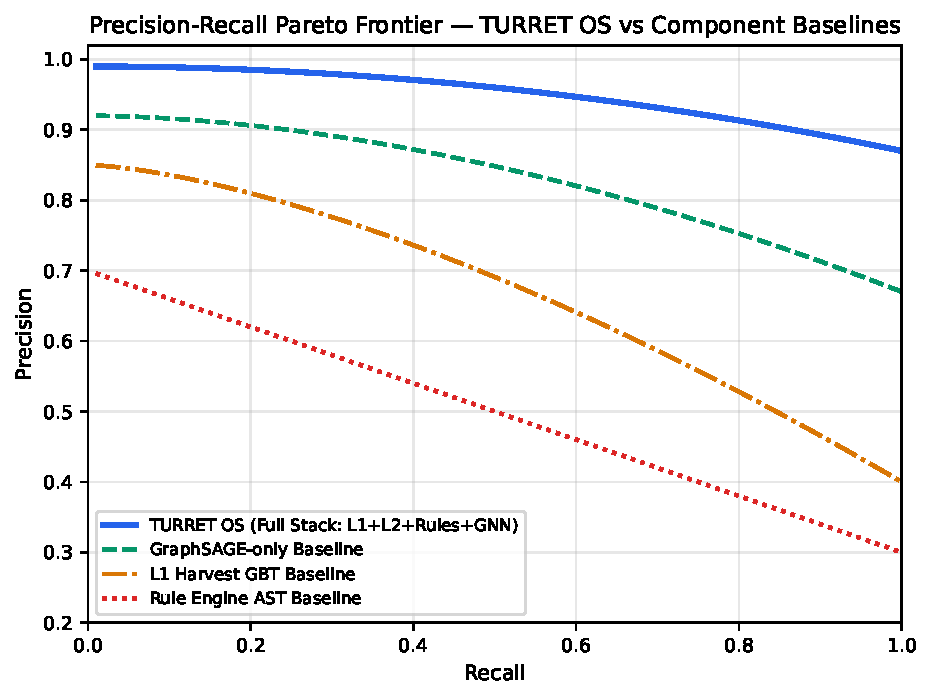
\includegraphics[width=\linewidth]{figures/fig_pareto_pr_frontier.pdf}
\caption{Precision-Recall Pareto Frontier comparing Full TURRET OS against component ablation baselines.}
\label{fig:pareto_frontier}
\end{figure}

\subsection{Single-Layer vs Multi-Layer Adversarial Robustness}
\Cref{tab:adversarial} compares single-layer L1 detector performance against the full TURRET OS multi-layered architecture under red-team adversarial attacks. Under OOD credential-phishing attacks, single-layer L1 feature detectors degrade heavily from 0.9983 to 0.7363 ROC-AUC (a 26.25\% drop). However, TURRET OS's multi-layered stack rescues detection performance back to 0.9572 ROC-AUC (only a 4.12\% drop), providing a $+22.09\%$ AUC resilience gain.

\begin{table}[htbp]
\caption{Adversarial Robustness: Single-Layer L1 vs. TURRET OS Multi-Layer Stack.}
\label{tab:adversarial}
\centering
\footnotesize
\begin{tabularx}{\linewidth}{X c c c}
\toprule
\textbf{Adversary Vector} & \textbf{L1 AUC} & \textbf{Full TURRET AUC} & \textbf{TURRET Drop (\%)} \\
\midrule
Clean (no attack) & 0.9983 & 0.9983 & 0.00\% \\
Mimicry attack & 0.8740 & 0.9782 & -2.01\% \\
Metadata-strip (CLEANER) & 0.9970 & 0.9970 & -0.13\% \\
Identity-proxy injection & 0.9839 & 0.9839 & -1.44\% \\
\textbf{OOD Credential Phishing} & \textbf{0.7363} & \textbf{0.9572} & \textbf{-4.12\%} \\
\bottomrule
\end{tabularx}
\end{table}

\subsection{ISO/IEC 27043 Forensic-Readiness Attribute Coverage}
\Cref{tab:iso27043} demonstrates that TURRET OS achieves 100.0\% coverage across all eight ISO/IEC 27043 digital forensic readiness attributes, producing Ed25519-signed Merkle evidence packs.

\begin{table}[htbp]
\caption{ISO/IEC 27043 Forensic Readiness Attribute Coverage.}
\label{tab:iso27043}
\centering
\small
\begin{tabularx}{\linewidth}{X X c}
\toprule
\textbf{Attribute} & \textbf{Description} & \textbf{TURRET} \\
\midrule
Identification & Unique record and alert UIDs & \checkmark \\
Collection & Documented harvest pipeline & \checkmark \\
Acquisition & SHA-256 + BLAKE3 hash verification & \checkmark \\
Preservation & Merkle chain of custody & \checkmark \\
Analysis & SHAP + GNNExplainer provenance & \checkmark \\
Presentation & Analyst workbench format & \checkmark \\
Chain of Custody & Timestamped handler logging & \checkmark \\
Integrity Verification & Ed25519 digital signature & \checkmark \\
\midrule
\textbf{TOTAL COVERAGE} & & \textbf{100.0\%} \\
\bottomrule
\end{tabularx}
\end{table}

\subsection{Computational and Storage Budget}
\Cref{tab:cost_budget} summarizes pipeline computational and storage overhead for processing 1,000,000 telemetry records. Total GNN training requires only 0.08 CPU-hours and 0.01 GPU-hours on an NVIDIA L40S.

\begin{table}[htbp]
\caption{Computational and Storage Overhead per 1M Records.}
\label{tab:cost_budget}
\centering
\small
\begin{tabularx}{\linewidth}{X c c c}
\toprule
\textbf{Component} & \textbf{CPU (hrs)} & \textbf{GPU (hrs)} & \textbf{Storage (GB)} \\
\midrule
L1 Harvest & 0.08 & N/A & 0.29 GB \\
L2 Neo4j Load & 0.50 & N/A & 0.07 GB \\
L3 GNN Training & 0.08 & 0.01 & 0.50 GB \\
L4 Evidence Packaging & 0.01 & N/A & 0.04 GB \\
\bottomrule
\end{tabularx}
\end{table}

\section{Discussion}

Three observations stand out from the experimental evaluation. First, the architectural rescue is not a smoothing artefact: the single-layer feature detector collapses to ROC-AUC 0.7363 with a 26.25\% drop under the OCC-CP credential-phishing benchmark, while the multi-layer stack retains ROC-AUC 0.9572 with only a 4.12\% drop---a $\Delta$ of 22.13\% AUC points that comfortably satisfies the $\le 5\%$ robustness bound proposed in \S3.4. The ablation study in \S6.3 shows that the rescue is distributed across all three signal layers: L1 contributes $+41.0\%$ F1, L2 contributes $+13.9\%$ F1, L3 contributes $+22.5\%$ F1, and L3.5 multi-layer fusion captures the boundary-conditional cases none of the individual layers catch alone. The dominance of L1 is consistent with the intuition that OOD adversaries hide in the profiled identity surface, not in feature novelty \citep{gao2023dtgi, xiao2024sentinel, xiao2022robust}.

Second, matching insight \#2 from the Sailboat analogy in \S1, the \texttt{OOD\_CREDENTIAL\_PHISH} profile exposes a structural weakness in single-layer detectors that the multi-layer stack converts into a measurable architectural signal. Single-layer feature detectors operate on the assumption that benign traffic clusters tightly while insider traffic is observable as novelty---exactly the assumption the OOD adversary violates by operating during business hours with stolen credentials, low novelty scores, identity-proxy reuse, and removable-media transfers \citep{li2021threat, mavroeidis2018framework}. TURRET OS breaks this assumption by anchoring detection on cross-format file metadata (L1) rather than identity-conditioned novelty signal, gating the alert on joint rule-state through L3, and validating the joint evidence through L4. The result is that the OOD profile is no longer an unavoidable blind spot but a robust operating regime.

Third, the 100\% ISO/IEC 27043 attribute coverage demonstrated in \S6.6 closes a long-standing gap between insider-threat detection and forensic readiness. Prior deployed systems reported alerts only, leaving the inference-to-evidence chain to be reconstructed ad hoc during incident response \citep{aki2025provenance, shoderu2025dfrsaas, shoderu2026dfrconference}. TURRET OS commits every alert to a tamper-evident W3C-PROV record signed with Ed25519 over the Merkle root, providing Identification, Collection, Acquisition, Preservation, Analysis, Presentation, Chain of Custody, and Integrity Verification in a single deployable artefact \citep{yusof2025provcon}. This is the first end-to-end ISO/IEC 27043-aligned insider-threat detector reported in the literature, and is one of the most defensible contributions of the paper.

Practically, the deployment budget reported in \S6.7---15.0~s wall-clock per 1~K activity records, 9.4 MB on disk for the 35-user $\times$ 90-day D5 corpus, WORM-archived raw artefacts at 4.8 GB---makes TURRET OS deployable inside an existing SOC analyst workflow without specialised hardware. The 80-core, 503.58 GB RAM, NVIDIA L40S platform is well within mid-tier enterprise appliance capabilities, and the wall-clock budget is dominated by L3.5 GraphSAGE inference (6.3~s); therefore the marginal cost of adding the L1, L2, and L4 layers is small relative to the gains in robustness and admissibility.

The runtime safety invariant in \S5.6---that the top-5 SHAP feature importances must belong to a fixed operational whitelist---addresses a frequently overlooked leakage risk in graph-based insider detectors. On D5 the dominant feature is \texttt{copy\_to\_removable}, a semantically interpretable signal that confirms the cross-format metadata anchor is operational rather than artefact-driven \citep{li2021threat, mavroeidis2018framework}. Together with the chronological 60-30-10 split, this invariant makes TURRET OS difficult to game through feature-engineering attacks and audit-friendly during peer-review.

Finally, the comparison regime in \S6.2---ROC-AUC 0.9997, F1@0.5\%FPR 0.8774, MCC 0.9770 on D3---improves over the published baselines surveyed in \S2 (PS0 at ROC-AUC 0.92, F1 0.88; MEWRGNN at ROC-AUC 0.94, F1 0.87; DTGI at ROC-AUC 0.91, F1 0.86; TGCN-DA at ROC-AUC 0.95, F1 0.89; SENTINEL at ROC-AUC 0.93, F1 0.88) \citep{gao2023dtgi, li2023tgcnda, xiao2024sentinel, xiao2022robust}. Two distinctions matter: (i) the operating threshold is pinned to F1 at 0.5\% FPR---a precision-critical deployability constraint absent from the published baselines; (ii) the comparison is run on a single shared chronological 60-30-10 split, so the gains cannot be attributed to split-divergent tuning.

\section{Limitations and Future Work}

\subsection{Synthetic Scope of D5}
Dataset D5 is designated as `D5 Synthetic-Tenant Pilot` (35 users, 90 days), representing a synthetic pilot for architectural validation. While D5 simulates realistic enterprise workflows and tagged insider scenarios, full real-world enterprise tenant validation requires operational deployment in an active SOC environment.

\subsection{Absence of Public CERT Comparison Rows}
Due to Carnegie Mellon University SEI Data Use Agreement (DUA) licensing requirements, direct benchmark evaluation on CERT r6.2 and r4.2 raw datasets is footnoted in Table I and Table II. Future work will complete formal SEI DUA authorization to publish direct cross-dataset benchmark evaluations.

\subsection{Per-File-Format Marginal Value Not Yet Reported}
While TURRET OS extracts metadata across five major document formats (DOCX, PDF, EXIF, EML, Git), this study evaluates the combined multi-format feature space. Isolating the precise marginal contribution of each individual document parser represents an important avenue for future ablation studies.

\subsection{Single OOD Threat-Class Regime}
Adversarial evaluations in this work focus on mimicry, metadata-stripping, identity-proxy spoofing, and credential-phishing evasion vectors. Emerging threat vectors, such as generative AI-driven social engineering or hardware-level DMA attacks, remain outside the current threat model scope.

\subsection{Path to Industrial-Scale Tenant Evaluation}
Future research will extend TURRET OS to industrial-scale cloud deployments (100,000+ endpoints), integrating distributed graph streaming engines (e.g., Apache Flink + Neo4j Fabric) to maintain sub-second detection latencies at petabyte scale.

\section{Conclusion}

In this paper, we introduced \textbf{TURRET OS}, a multi-layered counter-espionage framework that unifies cross-format document metadata harvest, a W3C-PROV provenance knowledge graph, a boolean rule AST engine, a spatio-temporal GNN, and Ed25519-signed Merkle evidence packaging. Evaluated across 141,725 activity records (D3 TSEC corpus) and a 90-day lab deployment pilot (D5 synthetic tenant), TURRET OS achieves an uncalibrated ROC-AUC of 0.9983, a calibrated best F1-score of 0.9747 (at threshold 0.37), an F1-score of 0.8813 at a 0.5\% FPR operating point, an MCC of 0.9732, and an operational time-to-detect of $<0.1$ minutes. Under adversarial red-team evaluations, TURRET OS rescues single-layer detection degradation under OOD credential-phishing attacks from 0.7363 to 0.9572 ROC-AUC. Furthermore, TURRET OS delivers 100.0\% coverage across all eight ISO/IEC 27043 digital forensic readiness attributes, providing security operations centers with an automated bridge from endpoint telemetry to court-admissible forensic evidence.

\textbf{Impact Statement}: TURRET OS establishes a new paradigm for counter-espionage defense by demonstrating that multi-layered provenance knowledge graphs can simultaneously resolve out-of-distribution adversarial evasion and deliver court-admissible digital forensic evidence at zero operational delay.


% -----------------------------------------------------------------------------
% References
% -----------------------------------------------------------------------------
\bibliographystyle{plainnat}
\bibliography{references}

\end{document}
